% LTeX: language=de-DE
\section{Virtuelle Maschine}

\begin{frame}{Etappen der Übersetzung: Code-Erzeugung}
	\begin{figure}[h]
		\begin{adjustbox}{max totalsize={\textwidth}{!},center}
			\begin{tikzpicture}[node distance=3mm and 1cm, inner sep=3mm]
				\node (syntactic_analysis_text) [inner sep=0] {Syntaxanalyse};
				\node (lexical_analysis) [rec, below=of syntactic_analysis_text] {Lexikalische Analyse};
				\node (syntactic_analysis) [rec, fit={(syntactic_analysis_text) (lexical_analysis)}] {};
				\node (semantic_analysis) [rec, right=of syntactic_analysis] {Semantische Analyse};
				\draw [arrow] (syntactic_analysis) -- (semantic_analysis);
				\node (codegen) [rec, fill=mLightBrown!35, right=of semantic_analysis] {Code-Erzeugung};
				\draw [arrow] (semantic_analysis) -- (codegen);
			\end{tikzpicture}
		\end{adjustbox}
	\end{figure}
\end{frame}

\begin{frame}{Virtuelle Maschine}
	\begin{itemize}
		\item<1-> Häufig: Eine \emph{Virtuelle Maschine} (VM) simuliert echte Computer
		      \begin{itemize}
			      \item Display
			      \item Lautsprecher
			      \item Festplatte
			      \item \dots
		      \end{itemize}
		\item<2-> Hier: Software, die wie die CPU eines Rechners funktioniert
	\end{itemize}
\end{frame}

\begin{frame}{Die rush VM}
	\begin{itemize}
		\item Führt ein zuvor übersetztes Programm aus
		\item Stackbasiertes Design
		\item Hoher Abstaktionsgrad
	\end{itemize}
\end{frame}

\begin{frame}{Felder der VM}
	\begin{description}
		\item<1->[stack] Für temporäre Werte
		\item<2->[mem] Für Variablen
		\item<2->[mem\_ptr] Für Speicherverwaltung
		\item<3->[call\_stack] Aufrufstapel (\emph{Befehlsähler} und \emph{Funktionszähler})
	\end{description}
\end{frame}

\begin{frame}{Struktur der Programme der rush VM}
	\begin{itemize}
		\item<1-> Unterteilung in Funktionen
		      \begin{itemize}
			      \item Ohne Namen
			      \item numerische Identifizierung
			      \item Enthält mehrere Anweisungen
		      \end{itemize}
		\item<2-> ca. 30 verschiedene Befehlscodes
		\item<3-> Struktur der Anweisungen: \enquote{\LirstInline{asm}{call 2}}
		      \begin{itemize}
			      \item<3-> Befehlscode (\texttt{call})
			      \item<3-> Optionaler Operand (\texttt{2})
		      \end{itemize}
	\end{itemize}
\end{frame}

\begin{frame}{Demonstration: Ein-/Ausgabe}
	\begin{minipage}{0.5\textwidth}
		\Lirsting[float=H, fancyvrb={frame=none, fontsize=\small}]{deps/paper/listings/fib.rush}
		\centering
		\Larrow{Ausgabe}
	\end{minipage}
	\hfill
	\begin{minipage}{0.35\textwidth}
		\Lirsting[float=H, fancyvrb={frame=none, fontsize=\footnotesize}, ranges={1-20,26-32}]{listings/vm_fib.s}
	\end{minipage}
\end{frame}

\begin{frame}{Demonstration: Laufzeitverhalten}
	\begin{figure}[H]
		\href{run:assets/01_rush_presentation_vm.mkv}{
			\movie{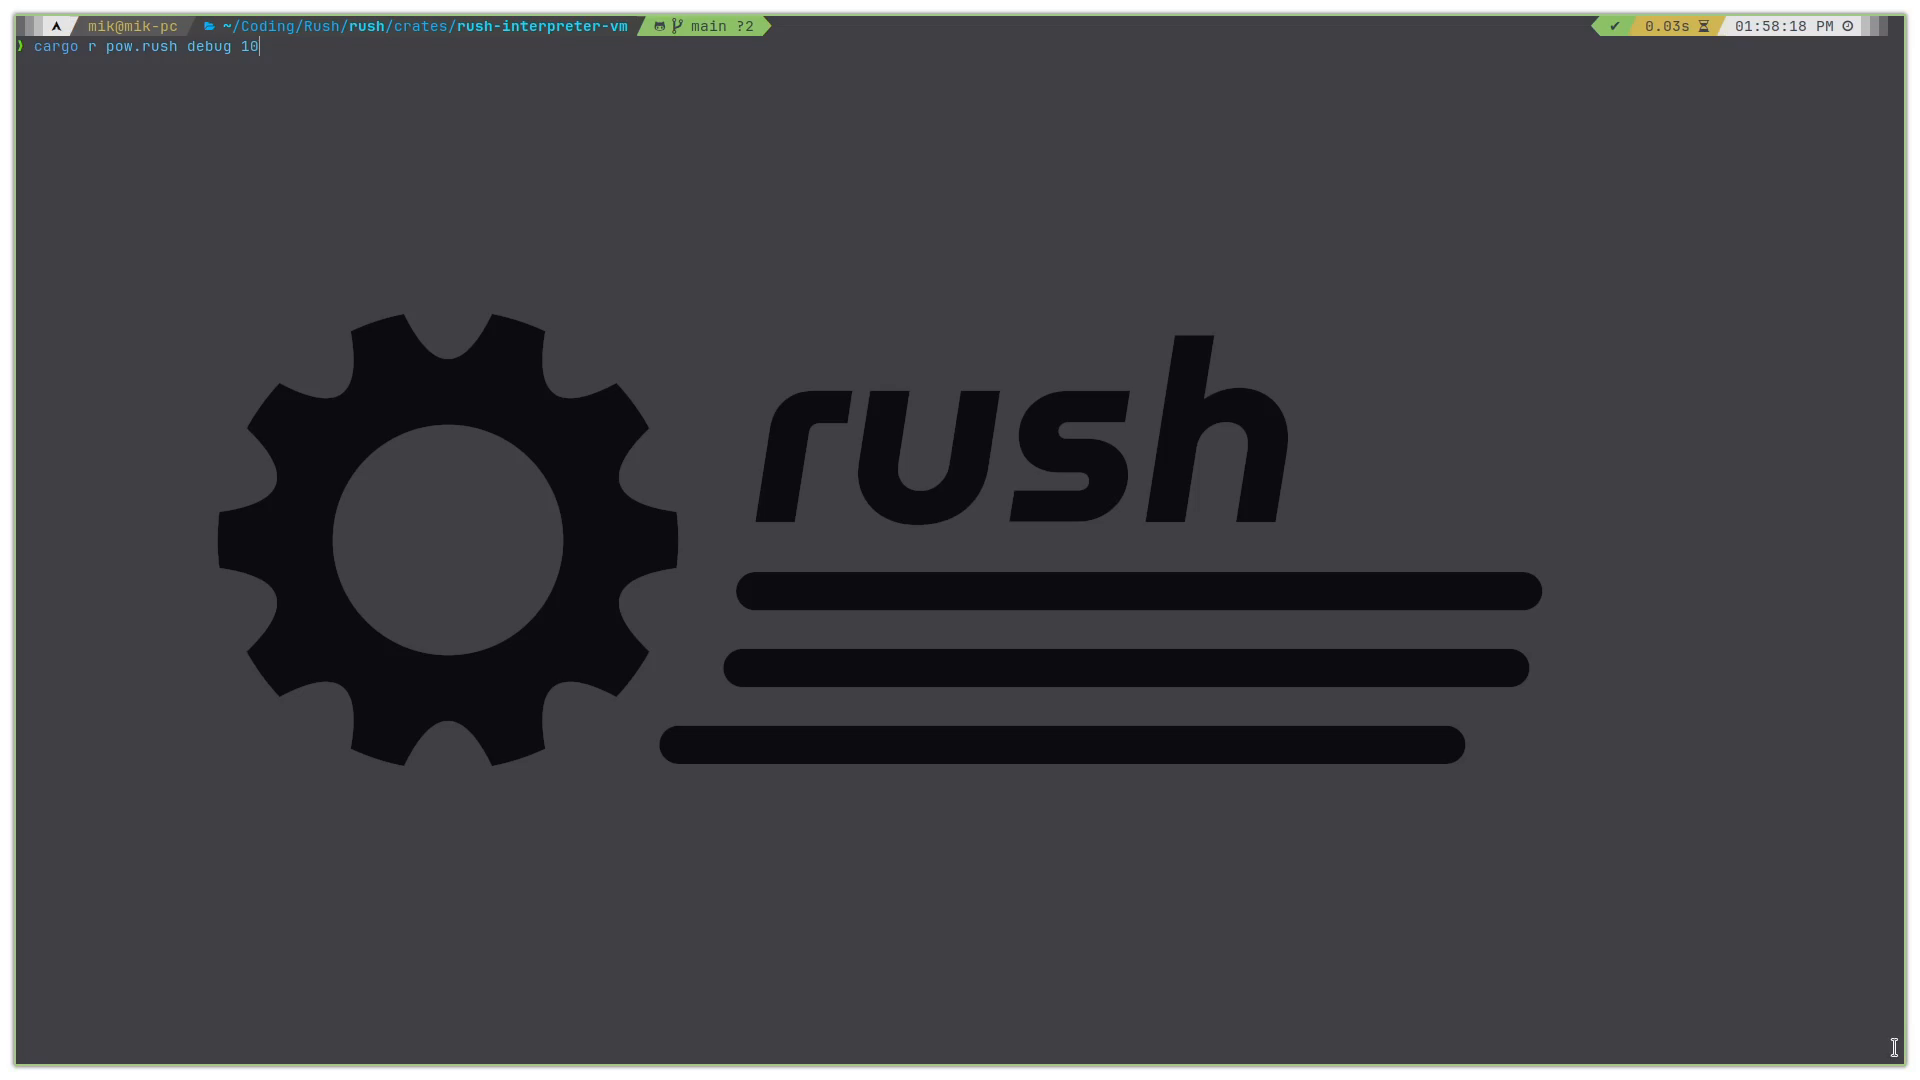
\includegraphics[width=.95\textwidth]{assets/01_rush_presentation_vm.png}}{assets/01_rush_presentation_vm.mkv}
		}
	\end{figure}
\end{frame}

\begin{frame}{VM: Fazit}
	\begin{itemize}
		\item<1-> Ca. 2.7 mal schneller als der Tree-walking Interpreter
		\item<2-> Einfache Implementierung des Compilers
			\begin{itemize}
				\item<3-> Stack-basierte Architektur
				\item<4-> Gleichzeitige Entwicklung von VM und Compiler (\cemph{Feedbackschleife})
				\item<5-> Hoher Abstraktionsgrad
			\end{itemize}
	\end{itemize}
\end{frame}
